\documentclass{amsart} \usepackage{amsmath} \usepackage{upgreek}
\usepackage{amssymb} \usepackage{graphicx}

\usepackage{enumerate} \usepackage[utf8]{inputenc}

\usepackage{tikz} \usepackage{hyperref}

\setlength{\textwidth}{6.37in} \setlength{\marginparwidth}{0pt}
\setlength{\evensidemargin}{0in} \setlength{\oddsidemargin}{0in}

\newtheorem{theorem}{Theorem}[section] \newtheorem{conj}[theorem]{Conjecture}

\newcommand{\x}[1]{\texttt{#1}}

\usepackage{titling} \setlength{\droptitle}{-8em}

\title{CS 452 Final Project \vspace{-0.65cm}} \date{Louis A. Burke (laburke) and
Taras V. Kolomatski (tkolomat)}

\begin{document}

\maketitle

\begin{center} \vspace{-0.58cm} July 28\textsuperscript{th}, 2017 \end{center}

\section*{The Program}

\textsc{Our} kernel development defined the possibilities of interactions of tasks in the real-time system. The blocks of our system, either tasks or constituent functions, are short elementary pieces of code, themselves non-monolithic. The first train control milestone produced the fundamental structural unit of the system - a tangled logic across tasks that accomplished the goal of controlling the movement of a train. The second train control milestone implemented protocols for the interaction of two of these fundamental units. This was accomplished by setting straightforward rules, lacking intricacy and far from optimal, to ensure the units interacted correctly - that the trains controlled did not collide. Thence the control of a single train is fundamental in the sense that its parts are not units of function, and that interaction among fundamental units is far more simple then their internal complexity.

\section*{Its Overview}

\textsc{We} have anthropomorphised the results of each previous assignment. Assignment zero was about the difficulty of communication. Kernel one was about how the context of human evolution, both biologically and sociologically, resulted in the equilibrium of society and control of its trajectory. Kernel two and three expended on the structure of this society and on the forces that must be counteracted to maintain it. Kernel four observed that the most successful communication was concise and simple.

Having produced the fundamental structural unit in the first train control milestone, we shifted away from the perspective of a human in the context of their society, to the perspective that society is just a byproduct of the inherent ingenuity of human thought. All interactions among people convey only an approximation of the complexity of the thoughts of their participants. The net effects of these sub-optimal manoeuvres could not possibly be the etiology of an individual's complexity.

\section*{The Theme}

Russian mathematician Israel Gelfand delivered a lecture for his receipt of the Kyoto prize, which honours the holistic contribution to humanity of the recipient's technical work. Titled, \textit{Two Archetypes in the Psychology of Man}, this lecture was on the the two conflicting human functions of wisdom and intellect. Wisdom is derived from experience, delivered to the individual by society. Intellect is ingenuity in fundamental opposition to the genetic and social conditioning of an individual, as observed from the patterns in society.

The outline of the lecture is as follows: Gelfand provides examples of the serious social conflicts that arise from the discrepancies of these views. This is the conflict of technocracy to the view of technology as evil, the conflict of illustrating the concept of a point to a student in saying that it is \textit{that which has no part}, appealing to intuition, and of taking a formal axiomatic approach that enforces rigour and eschews loose intuition, the conflict of a model to the reality that it is modeling - in all technical disciples (he speaks of his experience in biology, medicine, and computer science). He postulates that the cause of these conflicts is lack of an adequate language that can express both archetypes. For example, Hilbert showed that Euclidean geometry could be placed on fully rigorous ground. If one abandons the classic definition of a point, focusing only on axiomatic relations between a point and other geometric objects, one can purify the theory. Indeed one could take points to be classical planes, and planes to be classical points - the duality of projectile geometry does not care as three generic instances of one defines a unique instance of the other. A mathematician must have both intuitive and axiomatic understanding to conceive new results, hence, although the language differs, there is no fundamental divide between the views. Gelfand explains that mathematicians are capable to and responsible for producing such a language, which must describe the abstract notion of a fundamental unit: indivisible into complex systems, and interacting mutually in a far less complicated manner.

CS 452 is a course which clashes precise theoretical models with imperfect reality, the ability to perform any single task well with the requirement that necessarily less complicated protocols govern their interaction, and the creation of elegant, suddenly inspired, solutions with the inelegant and time consuming act of debugging. Computer science is a human field of study, and, in the course of these introductions, we have explained how the field's problems are reflections of a universal psychological dilemma fundamental to the human condition.

\section*{Calibration}

We know that steady state (no command related acceleration) velocity over a segment correlates well with distance traveled when stopping over the segment. In our first demo, we found these values by making a calibration loop every time we requested a train movement. We would record that the stop command be issued a certain number of ticks after a certain sensor activation. Further, we determined the progress of the train in the path it followed by counting sensor activations. Any sensor failures would be fatal to this approach, and it is not optimal to calibrate over the same segments multiple times.

We re-wrote the logic that determines progress in a path, identifying if an unusual sensor activation is the result of skipping a dead sensor. We further introduced a structure to store track calibration data. This structure records which sensors are dead and inter-sensor times. This structure allocates indexed space for storing records for all adjacent sensor pairs, and a constant number of entries for multiple segment times (with dead sensors in the middle). When running the program with no stored calibration data, we process a movement request as follows:
\begin{enumerate}[i.]
    \item We determine if the calibration data has times for every adjacent pair in the list of live sensors on the path (all of our paths are computed as circular, which eliminates the question of what to do in the case of dead endpoints).
    \item If there is insufficient data, then run the train on a calibration route.
    \item If there is sufficient data, calculate the stopping distance and find the last live sensor on the path that can serve as a trigger to stop after a delay (if the path is short and you think that, with few dead sensors, this would be a counterexample of the existence of such a sensor, then recall that all paths are circular).
\end{enumerate}
Because the map of path index to sensor ids is not necessarily injective on a circular path, the attribution logic mentioned above becomes relevant. Running over a calibration route fills in only records that do not already exist, dropping newer duplicate data. We don't loose generality by considering only circular routes without reversing, as this is a program only for calibration and maintaining steady state velocity over a track exit is impossible.

New calibration records were printed to the debug log, which was scp'ed over to our personal machines. We formatted the records to be the lines of C code that caused the records, and placed those code files in the \texttt{src/data} directory. There is a global macro to determine if the program is run in calibration mode. If it is set to false, then we run the code in \texttt{src/data}. If a calibration record does not exist at run-time, for example at the exits, then an average value is written into the structure.

\section*{Attribution and Reservation}

Our attribution and reservations systems are designed to be fairly simple, yet
parameterizable. This allows them to be robust, yet effective.

Our attribution system maintains the current and possible next sensors for each
train. If two trains are between two sensors then only the first one will
attribute to the destination, the second will only attribute there once the
first successfully passes it. Then when a sensor is flipped it iterates over all
of the trains in the system and decides if it was the one that flipped it. At
first it merely checks the immediately following sensors of each train. If after
that it can't find any match it will begin searching forward along both sensor
paths to see if the activated sensor might be one of the sensors after a dead
sensor. The distance ahead it looks is a specifiable constant.

Our reservation system is fairly straightforward, using a separate server to
request to own sections of track and route given other train's reservations. It
also provides the ability to steal sections of track to indicate that a train is
misbehaving. This notifies the previous owners of those sections and lets them
know that they may have to reroute. While this may not always prevent a
collision, it helps to at least provide a possible response to unexpected
behaviour.

An example of this is spurious sensor firings. The program can't determine which
train caused it, but must assume that something did, so it should route the
trains away from there - even though all trains were correctly told to avoid
that location. Similarly if a train moves too slowly and gets stuck at a
position on the track other trains will have to carefully route around it until
it is confirmed to have been removed.

\section*{Modularization}

In order to test many of the complicated subsystems in this assignment, we have
transferred most of our code to a separate directory and designing it to be
completely independent of our kernel and its systems. This allows us to unit
test this code on our own computers - helping to get tests done when there is a
lot of track contention.

\section*{Results}

Unfortunately when integrating the many systems involved in this assignment,
many kernel limitations were encountered which, coupled with heavy track
contention in the lab, resulted in a very unstable demo. While on rare
occassions the executable loaded would successfully dynamically avoid collisions
and deal with up to 4 simultaneous points of failure, for the most part it did
not perform as expected.

\section*{Moving Forward}

After adding extensive logs through the GUI to the project we have identified a
number of the problem sources and are slowly re-integrating each module one at a
time with extensive tests between each module's integration to ensure they work
well with previous modules. With new log systems in place bugs are much easier
to identify and development has become more streamlined.

\section*{Program Overview}

Prior to the development of modern drugs that are very effective in treating
epilepsy, severe cases warranted, with high efficacy, the surgical intervention
of a corpus callosotomy. In this procedure, the two hemispheres of the brain
were electrically isolated, effectively ceasing communication between the
preferential cortex of each hemisphere, resulting in a \textit{split brain}.

Such medical cases were of fervent interest to cognitive scientists, medical
researchers, and science fiction authors. One book that I enjoyed as a child,
\textit{Peace on Earth}, by Polish author Stanis\l{}aw Lem, involves a secret
held by a non-verbal and non-cooperative hemisphere of the protagonist's brain,
non-surgically divided by a blast from futuristic technology developed by
artificial intelligences continuing the Cold War on the moon. Lem portrays the
protagonist as having a \textit{split mind} - harbouring two separate
consciousnesses, with one controlling a hand that behaves much like that of
\textit{Doctor Strangelove} (Kubrick's film was released first).

However, this depiction is not accurate in the majority of cases. For example,
if two objects are placed each in the field of vision belonging to each
hemisphere (different eyes), then the patient will not be able to identify
whether the two objects are the same. This is expected - the test of equality
requires a complicated description to be conveyed between the hemispheres.
However, the hand controlled by each hemisphere will correctly indicate on paper
that an object is present in both visual fields. Further experiments revealed
that the rate of communication between hemispheres is approximately one bit per
second. This may result either by reading involuntary physical cues, or
emotional cues, consistently provided to both hemispheres by a shared
hind-brain. This limited communication allows patients to live a life with
little to no disability in the eyes of external observers.

We conceived of a project in which we would sever an initially present
networking link between the computers on which the terminals ran, representing
the surgery. Subsequently, the two tracks would communicate between each other
by choosing which train to send to the other track across a bridge we
constructed. These messages would be processed by passing through a network of
trains moving in periodic motion, and bringing the train to rest in an axon
opposite to the entry point, specific to the identity of the sent train.

\section*{Automatic Transmission}

The file \x{src/tasks/trains/transmission.c} contains the implementation of a
task that is responsible for issuing commands to adjust train speed to the
M\"arklin controller. One instance of the \x{transmission} task exists for each
active task. Aside from the routine involved in decoding the identity of a train
incoming across tracks, this task has sole agency for issuing commands to its
train.

The data stored in this task is a \x{speed\_combination}, which consists of two
speeds and two durations. The transmission task issues commands to alternate
between the two speeds at the specified durations. This struct is modified by
the \x{set\_speed} and \x{adjust\_speed} functions. It is maintained such that
the two speeds are adjacent integers within bounds, and such that the durations
are non-negative and sum to a defined number (in our demo, this was 15 ticks).
The gradation of steps by which one can adjust is also a defined number (in our
case 3).

The \x{transmission} task receives three types of commands: set, adjust, and
reverse. Delays are set by creating an asynchronous notifier such that the
transmission does not block and can receive other commands. This notifier
accounts for the fourth message type passed to the \x{transmission}. We chose to
kernel panic if a reverse command was issued while the speed was not set to
zero.

\section*{Defining a Schedule}

The file \x{src/util/trains/transit\_shcedule.c} contains the implementation for
\x{TransitSchedule}, the data structure for timed routes. It contains a
\x{RestrictedRoute}, a target velocity, an index of the last sensor visited, a
list of expected arrival times, a list of observed arrival times, and a train
number. Expectation values for sensors that have already been passed are
meaningful only if the route begins and ends at the same sensor node.

Given the \x{RestrictedRoute}, target velocity, initial sensor index, and
initial time, the expected times are defined at all future points in time. The
expected time values are obtained from the track data under the expectation that
the train will travel at the target velocity. The \x{init\_schedule\_times}
method prepares the schedule given this data.

Data entry is accomplished by the \x{transit\_register\_hit} function, which
takes a sensor id and time. This function will find the index of the sensor id
on the route, and will panic if this is an unreasonable attribution (not
explained by skipping fewer than three sensors on the route). When we said that
out final demo crashed once, we meant that a misattribution occurred and the
program returned to RedBoot. If the attribution is reasonable, this function
will record the time (marking any missed sensors), cyclically advance the
expected times (via a call to \x{rotate\_schedule}), log the observed times, and
return an integer representing the approximate distance deviation from the
schedule (obtained by multiplying the target velocity by the time delta).

Since this structure is responsible for logging time records, it also provides
the \x{transit\_vel\_from} function which provides velocity data over the
previous specified number of segments. Overall, this structure holds and
processes all the information that we need to make control decisions for trains
that follow a scheduled route.

\section*{Conforming to a Schedule}

The file \x{src/tasks/trains/conformist.c} contains three tasks:
\x{publicTrain}, \x{privateTrain}, and \x{conform}. The first two tasks are just
responsible for setting up a schedule and creating a \x{transmission} and
\x{conform}. (These tasks would initialize the schedules back by 2.5s to account
for acceleration.) The \x{conform} tasks survives for the duration of the demo
and is responsible for keeping a given train on a \x{TransitSchedule}. It
contains a parameter that allows for marking the end of a route - a feature used
by \x{privateTrain} to end the program after the messenger train arrives at the
target axon.

The \x{conform} task registers for sensor readings attributed to its train. It
registers these readings with its \x{TransitSchedule}, and uses the returned
distance deviation data and its requests for velocity data to make a decision of
which adjustments need to be sent to the train's \x{transmission}. The desired
behaviour is for a train to correct its deviations from the schedule and to soon
loose the information of its past deviation (errors dampen and we have a
guarantee of the \textit{ergodicity} hypothesis).

\vspace{0.4cm}

Let's trace through the development of this tasks and the performance
observations we made.

\vspace{0.4cm}

We began with the simplest behaviour that corrects for errors - increase
velocity if we are behind and decrease velocity if we are ahead (by a minimal
deviation threshold). We tested this on the route of track A's left circle.
On this route, different track segments are more equal relative to a more
diverse class of segment types, including straight ones, on other routes. We
observed that if distance deviations were less than 40cm (approximately less
than one second), then errors would dampen and deviation would oscillate with an
amplitude of approximately 30 cm. However, for larger errors, we would
repeatedly adjust the velocity many times before the deviation was corrected,
and the excess velocity would guarantee another deviation in the opposite
direction such that these errors would propagate and eventually result in a
collision. Moreover, when we repeated this experiment on a different route, we
saw that the non-uniformity of the track was sufficient to introduce
oscillations past the observed \textit{critical amplitude}.

Thus, we realized that, for example, if velocity data indicated that a train was
going 20cm / second over the target velocity while being behind schedule by 10
cm, then the correct action would be to decrease velocity to return to the
target velocity. We introduced a variable called \x{permissible\_bound}, which
gave bounds for acceptable velocity deviations, which was defined by a step
function given the error returned by the call to \x{transit\_register\_hit}.
This function was, with the argument in units of mm and the value in units of
mm/sec: \[ f(d) = \begin{cases} 20 & |d| \leq 40 \\ 50 & 40 <  |d| \leq 100 \\
100 & 100 < |d| \leq 300 \\ 150 & |d| > 300.  \end{cases} \]

The use of the \x{permissible\_bound} depended on whether the error was greater
than 50mm. For larger errors, we would read the velocity history from the last
segment, and if it was within the \x{permissible\_bound} (mono-directional -
i.e. we would only reject if the deviation was large and in the direction that
would result in correction), then we would issue a correction of at most three
ticks (0.6 speed integers) in the direction of correcting the distance error, as
a function of error. \textbf{\textit{After the demo we discovered an error in the
code}} - it was my intention to choose the number of ticks based on the
difference of the observed velocity and the sum of the target velocity and
bound, but we looked at the difference of observed velocity and the target
velocity. This contributed to over-correction in the demo and we would probably
have a much higher critical amplitude if this were corrected.

In the other case, errors less than or equal to 50mm or excess of the bound, we
would issue a single tick correction in the direction of the target velocity if
the bound was exceeded. On the route show in the demo, the critical amplitude
was 1m (about 2.5 seconds of deviation). We consistently saw that any
oscillations less than 70 cm would dampen to an oscillation of amplitude 15-30cm
(depending on the train). The non uniformity of the track, and our not
specifically accounting for it in the expected times, would always result in
deviations of the latter magnitude. This would happen within three passes of the
route. This was very within the bounds of tolerance for the demo and we were
happy.

Unfortunately, oscillations on the order of a metre would propagate. Prior to
the demo, we did not frequently observe errors of this magnitude. Something
happened to the track within the 45 min prior the demo - train 70 did not
previously get stuck at it's initial position and the deviation was entirely
unexpected! The program ran smoothly four times in a row prior to our demo. If
we would have observed this prior to the demo, then we would not have reset the
system and not sent the train over when we saw that train 70 experienced an
initial hiccup. We successfully twice demonstrated correct behaviour after three
failures (twice we sent the train over after a hiccup and once we experienced a
misattribution 30s after we began the program, causing a kernel panic and
graceful exit to RedBoot).

\section*{Passing a Train Through the Public Transportation System}

The \x{conform} tasks corresponding to the trains travelling in a circle
constitute the \textit{public transportation system} and are created on startup
by the \x{publicTrain} task. When a newly introduced train was decoded and
placed in its initial axon, we waited for 10s, and then launched the
\x{privateTrain} task to create a \x{transition} and \x{conform} for the new
train. Its route consisted of a fixed middle segment, appended to short
beginning and ending segments that would allow us to use different axons.

The \x{publicTrain} task faced the challenge of deciding at which delay to begin
the \x{TransitSchedule}. We made this decision via the \x{backtrace} function.
At time zero, we imagine a third \textit{spoke} in the public transportation
wheel at sensor E9, representing a hole. The \x{publicTrain} tasks would reply
to their creator with the period at which the route was completed. We thus have
a set of discrete times at which the hole is at sensor E9. The \x{privateTrain}
task chose the initial delay such that the expected arrival time of the
messenger train at sensor D10 (opposite E9 on the merge and very nearby)
coincided with the soonest point in this set that is achievable from the current
time.

We stopped the train a short while prior to arriving at the terminal axon, and,
after a delay, we issued the STOP command to the controller. This command was
indeed sent, but usually not correctly handled by the controller - the first
successful run in the demo was the only time that the command successfully
issued. Note that we delayed for 0.2s after issuing this command before
returning to RedBoot - we think that the error is endemic to the hardware,
related to processing this command while the controller is replying with sensor
readings.

\section*{Exitting and Scheduling}

During the first train control milestone, and persisting thereafter there were a
few bugs caused by exited tasks leaving behind problems. Once these bugs were
identified, the exit syscall was extended. This involved checking blocked tasks
to see if any are waiting on the exiting task to continue. In these cases their
intertask communication calls are aborted with the appropriate exit codes.

This also led to a slight modification of the scheduler and in general made us
aware of concurrency issues. In particular we realized that the server which
required the modification to be made could also cause a deadlock by sending to a
task trying to send back. In order to help ensure consistent communication
between tasks we created the following diagram of the major tasks to discover
where concurrency issues would have to be broken by a courier.

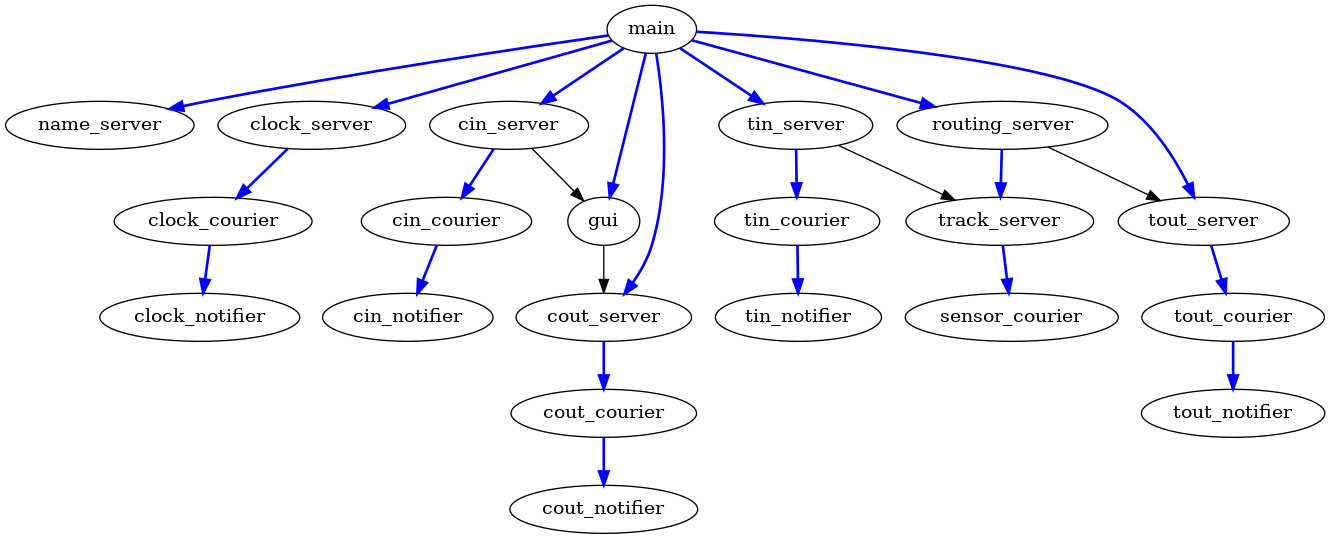
\includegraphics[width=\textwidth]{../src/tasks.png}

After analyzing the earlier form of said diagram, a cyclic dependency was
discovered with respect to the \x{gui} task and the \x{track\_server} task. This
dependency was broken by special courier allocation and reordering creation of
tasks.

\section*{Regrets}

The main aspect of our code that we regret is our focus on performance. Given
the emphasis on performance and competitive nature of our team members, we
strived to produce the most performant code possible, and this sometimes meant
that robustness was a secondary concern. You may note that performance is listed
below as one of the things of which we are most proud. This is still true. We
are proud of our performance, but wish that we could have had more robustness as
well.

Some of the areas in which more robustness could have been helpful are as
follows.

\begin{itemize}
    \item Return codes - We rarely check the return codes of our syscalls except
        where necessary. We could have found some of our bugs early had we
        maintained a policy of checking all syscall return values.

    \item Message passing - Many of our bugs have been due to poorly formed or
        received messages. A large proportion of the messages we send are
        zero-sized (for performance) with their meaning determined from the
        sender's tid, or merely the fact that the message has no size. However
        this makes it impossible to detect and recover from an error, as if a
        task sends zero bytes to a server waiting to hear it, there is no way
        for that server to realize it has the wrong message. Ideally we would
        tag each message with some unique value and sanity check every received
        message to ensure that the message received is from where we expect.

    \item Array bounds - As a lot of our most difficult bugs came from
        addressing off the end of an array, it would have been beneficial to
        create a robust array data type which we could use to ensure that we
        never access memory we don't have access to.

    \item General robustness - A lot of our code was not designed with failure
        in mind. The above cases are merely symptoms of overall code quality.
        While our code has very good performance qualities, it sacrifices
        robustness. For example many functions which could cause errors merely
        cause a kernel panic rather than trying to address them or returning
        some error code. Many functions also assume their data has a certain
        format without indicating as such with a comment or checking that it is
        the case. In general we have zero run-time assertions in place. The
        result is that large-scale bugs can be nearly impossible to diagnose.
\end{itemize}

The final regret is that our reservation system (the Hotel) never became fully
operational. While it worked on its own as a unit, the use of it resulted in
many concurrency bugs that made integrating it not worthwhile. Even the GUI had
the ability to draw which sections were reserved, but this was never used as our
code never reserved any sections.

\section*{Of What we are Most Proud}

\subsection*{Performance}

We put a lot of effort and very specific knowledge into optimizing the raw
performance of our kernel. We were able to get our Send/Receive/Reply cycle down
to just under 8 microseconds in the optimal case. This meant that we never
really ran into significant performance problems while working on the project,
freeing us up to focus on more difficult problems.

One way in which we improved performance was by moving to a newer compiler, so
as to generate more optimized code. We also carefully optimized performance
critical sections of code, such as the scheduler. One of the most useful little
things we did was to manually organize the linker script so that critical
segments of code appeared near each other. Once caches were turned on, this
caused significant improvement in performance by reducing some cache misses.

\subsection*{HWIs do not trap into the kernel}

We reserved 100 words of space at the top of the kernel stack for processing
hardware interrupts and did not context switch into the frame of the kernel.
Further, the HWI event did not even call code that we wrote in assembly for
context switching - the HWI handler was short, simple, and inlined, such that
the compiler directive \x{\_\_attribute\_\_((interrupt("IRQ")))}, would save and
restore exactly the registers that it clobbered, and would call the \x{movs}
instruction at return!  The HWI handler's behaviors was to disable the interrupt
by masking it away on the CPU (not at all dealing with the memory mapped
locations that resulted in its issue) and unblocking the event handler in the
scheduler. The latter did not cause re-scheduling and we were guaranteed
atomicity between syscalls in user space tasks. Without this, for example, the
debug log that we wrote to in memory would be susceptible to a race condition
that would intersperse logs at best, and insert or remove a null-terminator at
worst.

\subsection*{Scheduling}

Despite the guidelines of the course, we wrote a slightly fairer scheduler than
the raw round-robin priority first based scheduler. Our scheduler does a bit
more work to allow lower priority tasks to on occasion execute even if a higher
priority task is waiting. This does not prevent that task from executing, but
rather has it execute more frequently then the lower priority tasks. In
addition, we have real-time priority tasks which are guaranteed to execute
whenever possible and before any higher priority task.

This allowed us to essentially ignore priorities while developing our solutions
for the project. In general we gave more important tasks higher priorities and
less important tasks lower priorities, but we didn't overly concern ourselves
with exactly which priorities were given to which tasks. This is because even if
an important task has a lower priority than another task, it doesn't mean it
can't ever execute, it just executes less. Given that the vast majority of our
execution occurs as a direct response to an interrupt, most tasks are left to
execute in exactly the order of their priorities. However, if we were to
accidentally create priorities such that a task would be starved, it would not
be, it would merely run less often. This relieved a lot of the pressure to
carefully pick task priorities.

\subsection*{The stopping model}

Stopping models based on physics are placed on incorrect foundation, as taking
the train to a stop is actually an illusion handled by software - cutting power
to the track results in the same observable behaviour as suddenly issuing a
reverse command. The goal, thus, is to fit to a function of the correct
parameters. We discovered a remarkably tight fit to steady state velocity over
the segments on which the stop would occur. More surprisingly, we discovered a
inverse correlation within each speed setting of stopping distance to incoming
velocity! This is because there is a negative correlation between steady state
velocity on adjacent segments. We have concluded that this is caused by the
placement of switches at approximately every second segment, as we have
observed, with a voltmeter, that one section of rail in each switch does
not provide power. The implication of this is that if a TC1 demo is made all in
one speed setting, then determining stopping distance from the overall
regression values applied to incoming velocity is strictly worse than using a
constant value.

\subsection*{GUI}

We created a true Graphical User Interface (GUI) in Ada by directly listening to
the com port on the more powerful desktop computers in the lab. This allowed us
to provide a more intuitive and powerful interface than a mere text-based UI
could offer. While the introduction of a GUI caused a few bugs to present
themselves, and took some time from possibly more critical features, it also
unlocked powerful debugging opportunities. For example, the GUI allowed for
logs to be collected more efficiently than merely dumping them to the screen
during runtime.

\subsection*{Logs}

The GUI was not the only system we used to collect logs. We also used an atomic
log based system for debugging. This worked by writing a large null-terminated
string directly into the ts7200's memory in a location that was largely unused.
In particular we stored the log from address 0x50000 (only a few kilobytes from
the top of RedBoot) to address 0x100000 (the first byte of our kernel). These
could then be retrieved and read after the program completed by a separate
logging program. Thus we could pump massive amounts of information into logs
during performance critical sections of code without having to wait for the
console UART interrupts and various task reschedulings. Additionally we could
debug things at a lower level, such as scheduler progress and kernel
information. These could not possibly be printed to the screen as that would
require that they communicate with the I/O tasks.

\subsection*{Structure}

The final thing about which we are proud is our code organization. Throughout
the project we have strived to maintain a consistent organized file structure
and avoid monolithic files. While many groups ended up with multi-thousand line
files for some of the more powerful servers (like the train/track state
maintenance server), we carefully modularized our code into small testable
files. This helped greatly with debugging.

\section*{SHA of commits}

\textsc{Now} that the project is done, everything is being pushed up to the git
repo. As such the entire repository is effectively our submission. The actual
code used exists on two branches. The UI used in the demo was created on the
\texttt{dev-logging} branch with hash
\texttt{1a80be424be4ab79a05807acb2cb2579319d5d00}. The public transit protocol
was created on the \texttt{final-demo} branch with hash
\texttt{d67465d1279f2058a1f9f86723930b34956fa389}.

\noindent The repository can be cloned from:

\url{gitlab@git.uwaterloo.ca:laburke/cs452_kernel.git} (SSH)

or

\url{https://git.uwaterloo.ca/laburke/cs452_kernel.git} (HTTPS)

\textbf{There is a README in the root directory of the repository which outlines
the loading command.} To run the program once it is compiled just restart the
machine and run \[\texttt{load -h 10.15.167.5 "ARM/user/kernel.elf"}\] to load
it.
\end{document}
